\documentclass{standalone}
\usepackage{tikz}
\begin{document}
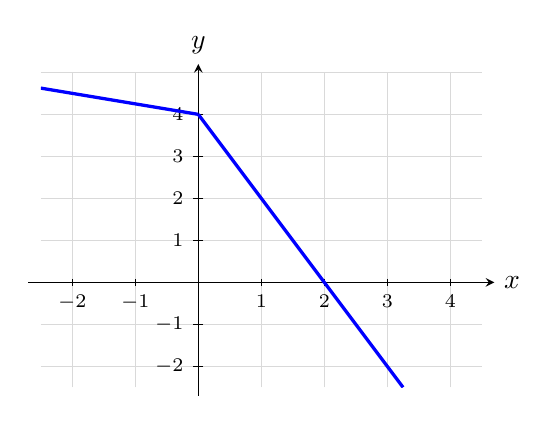
\begin{tikzpicture}[>=stealth, scale=0.8, yscale=2/3]
  % Gridlines
  \draw[very thin, gray!30] (-2.5,-2.5) grid (4.5,5);

  % Axes
  \draw[->] (-2.7,0) -- (4.7,0) node[right] {$x$};
  \draw[->] (0,-2.7) -- (0,5.2) node[above] {$y$};

  % x-axis tick labels
  \foreach \x in {-2,-1,1,2,3,4}
    \draw (\x,0.08) -- (\x,-0.08) node[below, font=\scriptsize] {$\x$};
  % y-axis tick labels
  \foreach \y in {-2,-1,1,2,3,4}
    \draw (0.08,\y) -- (-0.08,\y) node[left, font=\scriptsize] {$\y$};

  % Function curve (piecewise linear, continuous corner at (0,4))
  \begin{scope}
    \clip (-2.5,-2.5) rectangle (4.5,5);
    % Left piece: slope -1/4 through (0,4)
    \draw[blue, very thick] (-2.5,4.625) -- (0,4);
    % Right piece: slope -2 through (0,4), x-intercept at (2,0)
    \draw[blue, very thick] (0,4) -- (3.25,-2.5);
  \end{scope}
\end{tikzpicture}
\end{document}
